% Options for packages loaded elsewhere
\PassOptionsToPackage{unicode}{hyperref}
\PassOptionsToPackage{hyphens}{url}
\PassOptionsToPackage{dvipsnames,svgnames,x11names}{xcolor}
%
\documentclass[
  authoryear,
  preprint,
  3p]{elsarticle}

\usepackage{amsmath,amssymb}
\usepackage{lmodern}
\usepackage{iftex}
\ifPDFTeX
  \usepackage[T1]{fontenc}
  \usepackage[utf8]{inputenc}
  \usepackage{textcomp} % provide euro and other symbols
\else % if luatex or xetex
  \usepackage{unicode-math}
  \defaultfontfeatures{Scale=MatchLowercase}
  \defaultfontfeatures[\rmfamily]{Ligatures=TeX,Scale=1}
\fi
% Use upquote if available, for straight quotes in verbatim environments
\IfFileExists{upquote.sty}{\usepackage{upquote}}{}
\IfFileExists{microtype.sty}{% use microtype if available
  \usepackage[]{microtype}
  \UseMicrotypeSet[protrusion]{basicmath} % disable protrusion for tt fonts
}{}
\makeatletter
\@ifundefined{KOMAClassName}{% if non-KOMA class
  \IfFileExists{parskip.sty}{%
    \usepackage{parskip}
  }{% else
    \setlength{\parindent}{0pt}
    \setlength{\parskip}{6pt plus 2pt minus 1pt}}
}{% if KOMA class
  \KOMAoptions{parskip=half}}
\makeatother
\usepackage{xcolor}
\setlength{\emergencystretch}{3em} % prevent overfull lines
\setcounter{secnumdepth}{5}
% Make \paragraph and \subparagraph free-standing
\ifx\paragraph\undefined\else
  \let\oldparagraph\paragraph
  \renewcommand{\paragraph}[1]{\oldparagraph{#1}\mbox{}}
\fi
\ifx\subparagraph\undefined\else
  \let\oldsubparagraph\subparagraph
  \renewcommand{\subparagraph}[1]{\oldsubparagraph{#1}\mbox{}}
\fi

\usepackage{color}
\usepackage{fancyvrb}
\newcommand{\VerbBar}{|}
\newcommand{\VERB}{\Verb[commandchars=\\\{\}]}
\DefineVerbatimEnvironment{Highlighting}{Verbatim}{commandchars=\\\{\}}
% Add ',fontsize=\small' for more characters per line
\usepackage{framed}
\definecolor{shadecolor}{RGB}{241,243,245}
\newenvironment{Shaded}{\begin{snugshade}}{\end{snugshade}}
\newcommand{\AlertTok}[1]{\textcolor[rgb]{0.68,0.00,0.00}{#1}}
\newcommand{\AnnotationTok}[1]{\textcolor[rgb]{0.37,0.37,0.37}{#1}}
\newcommand{\AttributeTok}[1]{\textcolor[rgb]{0.40,0.45,0.13}{#1}}
\newcommand{\BaseNTok}[1]{\textcolor[rgb]{0.68,0.00,0.00}{#1}}
\newcommand{\BuiltInTok}[1]{\textcolor[rgb]{0.00,0.23,0.31}{#1}}
\newcommand{\CharTok}[1]{\textcolor[rgb]{0.13,0.47,0.30}{#1}}
\newcommand{\CommentTok}[1]{\textcolor[rgb]{0.37,0.37,0.37}{#1}}
\newcommand{\CommentVarTok}[1]{\textcolor[rgb]{0.37,0.37,0.37}{\textit{#1}}}
\newcommand{\ConstantTok}[1]{\textcolor[rgb]{0.56,0.35,0.01}{#1}}
\newcommand{\ControlFlowTok}[1]{\textcolor[rgb]{0.00,0.23,0.31}{#1}}
\newcommand{\DataTypeTok}[1]{\textcolor[rgb]{0.68,0.00,0.00}{#1}}
\newcommand{\DecValTok}[1]{\textcolor[rgb]{0.68,0.00,0.00}{#1}}
\newcommand{\DocumentationTok}[1]{\textcolor[rgb]{0.37,0.37,0.37}{\textit{#1}}}
\newcommand{\ErrorTok}[1]{\textcolor[rgb]{0.68,0.00,0.00}{#1}}
\newcommand{\ExtensionTok}[1]{\textcolor[rgb]{0.00,0.23,0.31}{#1}}
\newcommand{\FloatTok}[1]{\textcolor[rgb]{0.68,0.00,0.00}{#1}}
\newcommand{\FunctionTok}[1]{\textcolor[rgb]{0.28,0.35,0.67}{#1}}
\newcommand{\ImportTok}[1]{\textcolor[rgb]{0.00,0.46,0.62}{#1}}
\newcommand{\InformationTok}[1]{\textcolor[rgb]{0.37,0.37,0.37}{#1}}
\newcommand{\KeywordTok}[1]{\textcolor[rgb]{0.00,0.23,0.31}{#1}}
\newcommand{\NormalTok}[1]{\textcolor[rgb]{0.00,0.23,0.31}{#1}}
\newcommand{\OperatorTok}[1]{\textcolor[rgb]{0.37,0.37,0.37}{#1}}
\newcommand{\OtherTok}[1]{\textcolor[rgb]{0.00,0.23,0.31}{#1}}
\newcommand{\PreprocessorTok}[1]{\textcolor[rgb]{0.68,0.00,0.00}{#1}}
\newcommand{\RegionMarkerTok}[1]{\textcolor[rgb]{0.00,0.23,0.31}{#1}}
\newcommand{\SpecialCharTok}[1]{\textcolor[rgb]{0.37,0.37,0.37}{#1}}
\newcommand{\SpecialStringTok}[1]{\textcolor[rgb]{0.13,0.47,0.30}{#1}}
\newcommand{\StringTok}[1]{\textcolor[rgb]{0.13,0.47,0.30}{#1}}
\newcommand{\VariableTok}[1]{\textcolor[rgb]{0.07,0.07,0.07}{#1}}
\newcommand{\VerbatimStringTok}[1]{\textcolor[rgb]{0.13,0.47,0.30}{#1}}
\newcommand{\WarningTok}[1]{\textcolor[rgb]{0.37,0.37,0.37}{\textit{#1}}}

\providecommand{\tightlist}{%
  \setlength{\itemsep}{0pt}\setlength{\parskip}{0pt}}\usepackage{longtable,booktabs,array}
\usepackage{calc} % for calculating minipage widths
% Correct order of tables after \paragraph or \subparagraph
\usepackage{etoolbox}
\makeatletter
\patchcmd\longtable{\par}{\if@noskipsec\mbox{}\fi\par}{}{}
\makeatother
% Allow footnotes in longtable head/foot
\IfFileExists{footnotehyper.sty}{\usepackage{footnotehyper}}{\usepackage{footnote}}
\makesavenoteenv{longtable}
\usepackage{graphicx}
\makeatletter
\def\maxwidth{\ifdim\Gin@nat@width>\linewidth\linewidth\else\Gin@nat@width\fi}
\def\maxheight{\ifdim\Gin@nat@height>\textheight\textheight\else\Gin@nat@height\fi}
\makeatother
% Scale images if necessary, so that they will not overflow the page
% margins by default, and it is still possible to overwrite the defaults
% using explicit options in \includegraphics[width, height, ...]{}
\setkeys{Gin}{width=\maxwidth,height=\maxheight,keepaspectratio}
% Set default figure placement to htbp
\makeatletter
\def\fps@figure{htbp}
\makeatother

\newpageafter{author}
\makeatletter
\makeatother
\makeatletter
\makeatother
\makeatletter
\@ifpackageloaded{caption}{}{\usepackage{caption}}
\AtBeginDocument{%
\ifdefined\contentsname
  \renewcommand*\contentsname{Table of contents}
\else
  \newcommand\contentsname{Table of contents}
\fi
\ifdefined\listfigurename
  \renewcommand*\listfigurename{List of Figures}
\else
  \newcommand\listfigurename{List of Figures}
\fi
\ifdefined\listtablename
  \renewcommand*\listtablename{List of Tables}
\else
  \newcommand\listtablename{List of Tables}
\fi
\ifdefined\figurename
  \renewcommand*\figurename{Figure}
\else
  \newcommand\figurename{Figure}
\fi
\ifdefined\tablename
  \renewcommand*\tablename{Table}
\else
  \newcommand\tablename{Table}
\fi
}
\@ifpackageloaded{float}{}{\usepackage{float}}
\floatstyle{ruled}
\@ifundefined{c@chapter}{\newfloat{codelisting}{h}{lop}}{\newfloat{codelisting}{h}{lop}[chapter]}
\floatname{codelisting}{Listing}
\newcommand*\listoflistings{\listof{codelisting}{List of Listings}}
\makeatother
\makeatletter
\@ifpackageloaded{caption}{}{\usepackage{caption}}
\@ifpackageloaded{subcaption}{}{\usepackage{subcaption}}
\makeatother
\makeatletter
\@ifpackageloaded{tcolorbox}{}{\usepackage[many]{tcolorbox}}
\makeatother
\makeatletter
\@ifundefined{shadecolor}{\definecolor{shadecolor}{rgb}{.97, .97, .97}}
\makeatother
\makeatletter
\makeatother
\journal{Ecological Informatics}
\ifLuaTeX
  \usepackage{selnolig}  % disable illegal ligatures
\fi
\usepackage[]{natbib}
\bibliographystyle{elsarticle-harv}
\IfFileExists{bookmark.sty}{\usepackage{bookmark}}{\usepackage{hyperref}}
\IfFileExists{xurl.sty}{\usepackage{xurl}}{} % add URL line breaks if available
\urlstyle{same} % disable monospaced font for URLs
\hypersetup{
  pdftitle={Parr and Spawner Abundances of Sockeye Salmon (Oncorynchus nerka) from Osoyoos Lake (British Columbia, Canada).},
  pdfauthor={Scott A. Akenhead; Braden Judsen},
  pdfkeywords={Sockeye Salmon, Osoyoos Lake, Oncorynchus nerka},
  colorlinks=true,
  linkcolor={blue},
  filecolor={Maroon},
  citecolor={Blue},
  urlcolor={Blue},
  pdfcreator={LaTeX via pandoc}}

\setlength{\parindent}{6pt}
\begin{document}

\begin{frontmatter}
\title{Parr and Spawner Abundances of Sockeye Salmon (Oncorynchus nerka)
from Osoyoos Lake (British Columbia, Canada).}
\author[1]{Scott A. Akenhead%
\corref{cor1}%
\fnref{fn1}}
 \ead{scott@s4s.com} 
\author[1]{Braden Judsen%
%
\fnref{fn2}}
 \ead{braden.judsen@dfo-mpo.gc.ca} 

\affiliation[1]{organization={Pacific Biological Station, Fisheries and
Oceans Canada},addressline={3190 Hammond Bay
Road},city={Nanaimo},postcode={V9T 6N7},postcodesep={}}

\cortext[cor1]{Corresponding author}
\fntext[fn1]{This is the first author footnote.}
\fntext[fn2]{Another author footnote, this is a very long footnote and
it should be a really long footnote. But this footnote is not yet
sufficiently long enough to make two lines of footnote text.}
        
\begin{abstract}
We analysed 106 (?) surveys, from the 27 years 1996--2022, of parr, the
lacustrine life stage of Sockeye Salmon, in small, warm, and eutrophic
Osoyoos Lake in the Columbia River watershed. All the surveys were
aggregated for a regression to determine annual abundance and the
pattern of mortality rate through this life stage. That regression
provided abundance estimates for each year at standardized dates
representing beginning and end of that life stage. Attention to (a) the
relative precision of each survey as regression weights, and (b) factors
known to affect parr survival (flows, a pollution event, parr size)
improved the precision of estimates. The parents of these parr were
surveyed repeatedly each year as spawners in the Okanagan River
immediately upstream of Osoyoos Lake. A spawners to early parr
regression similarly benefited by including river flows as a factor
known to affect egg, alevin, and migrating fry survival. Given that
spawners predict early parr, thus inform parr abundance, we merged these
two models to determine how shared information might benefit both.
\ldots{} and then what? Don't stop there! What the hell?
\end{abstract}





\begin{keyword}
    Sockeye Salmon \sep Osoyoos Lake \sep 
    Oncorynchus nerka
\end{keyword}
\end{frontmatter}
    \ifdefined\Shaded\renewenvironment{Shaded}{\begin{tcolorbox}[frame hidden, interior hidden, borderline west={3pt}{0pt}{shadecolor}, sharp corners, enhanced, boxrule=0pt, breakable]}{\end{tcolorbox}}\fi

\hypertarget{doc-prep-notes}{%
\subsubsection{Doc Prep Notes}\label{doc-prep-notes}}

\url{https://www.elsevier.com/authors/policies-and-guidelines/latex-instructions}
styles

Here are \citep{hyatt2015} example citations
\citep{fryer2018, fryer2011} from Zotero shared library:
\href{https://www.zotero.org/groups/4787789/okanagan_sockeye_2023/library}{Okanagan
Sockeye 2023.}

Here is an equation the ref is Equation~\ref{eq-lorenz} and that
resulted in a numbered equation.
\begin{equation}\protect\hypertarget{eq-lorenz}{}{ 
  f_{X}(x) = \left(\frac{\alpha}{\beta}\right)
  \left(\frac{x}{\beta}\right)^{\alpha-1}
  e^{-\left(\frac{x}{\beta}\right)^{\alpha}}; 
  \alpha,\beta,x > 0 .
}\label{eq-lorenz}\end{equation}

Inline equations work as well: \(\sum_{i = 2}^\infty\{\alpha_i^\beta\}\)

This is @fig-meaningless from an R chunk. Does each fig and table need
separate chunk? The journal format move pictures to end but not figures
and tables from R chunks?

\begin{figure}

{\centering 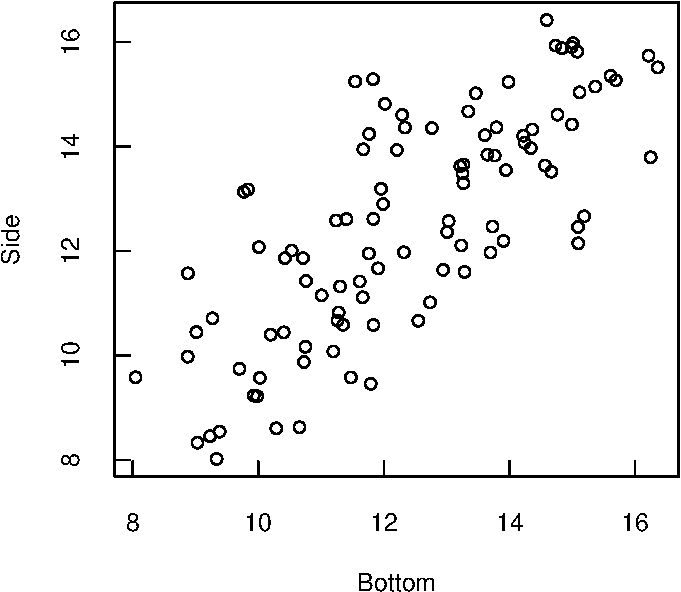
\includegraphics[width=0.5\textwidth,height=\textheight]{OSO-Parr-Primary_files/figure-pdf/fig-meaningless-1.pdf}

}

\caption{\label{fig-meaningless}Samples from a bivariate normal
distribution.}

\end{figure}

\hypertarget{pictures}{%
\subsubsection{Pictures}\label{pictures}}

Just use \textbf{\texttt{Insert}} in Quatro Visual, then adjust size
after. This picture is referenced from
\texttt{Attributes\ \textgreater{}\textgreater{}\ ID\ \#fig-paths}.
Journal format automatically moves pictures to end. (!)

\begin{figure}

{\centering 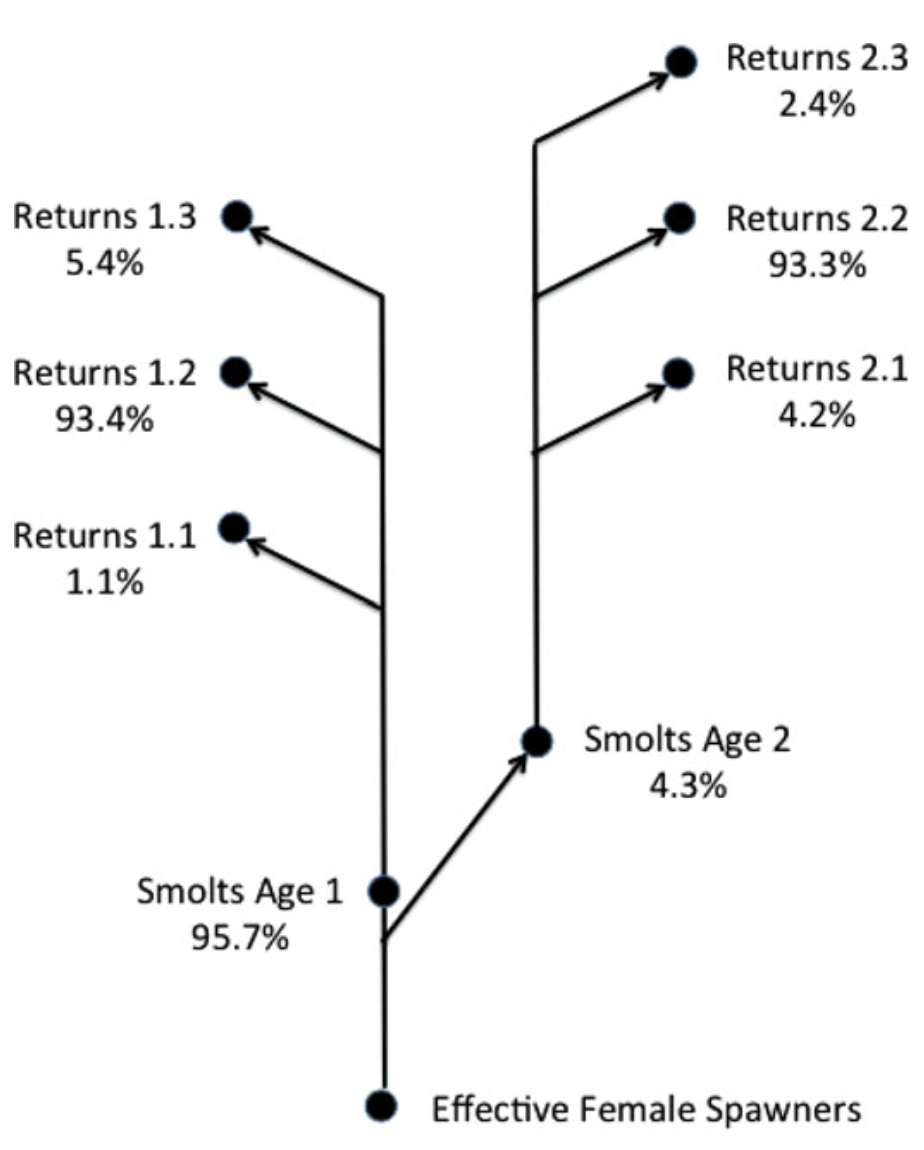
\includegraphics[width=3.20833in,height=\textheight]{example_image.png}

}

\caption{\label{fig-paths}Life Paths of Chilko sockeye. Each cohort is
observed nine times over 6 years. Percentages are the mean values from
1960--2008.}

\end{figure}

\hypertarget{tables-from-r}{%
\subsubsection{Tables from R}\label{tables-from-r}}

Caption and label (for reference) in chunk, here is
Table~\ref{tbl-simple} as an example.

\begin{Shaded}
\begin{Highlighting}[]
\NormalTok{knitr}\SpecialCharTok{::}\FunctionTok{kable}\NormalTok{(}\FunctionTok{head}\NormalTok{(mtcars)[,}\DecValTok{1}\SpecialCharTok{:}\DecValTok{4}\NormalTok{])}
\end{Highlighting}
\end{Shaded}

\hypertarget{tbl-simple}{}
\begin{longtable}[]{@{}lrrrr@{}}
\caption{\label{tbl-simple}Caption centered above table}\tabularnewline
\toprule()
& mpg & cyl & disp & hp \\
\midrule()
\endfirsthead
\toprule()
& mpg & cyl & disp & hp \\
\midrule()
\endhead
Mazda RX4 & 21.0 & 6 & 160 & 110 \\
Mazda RX4 Wag & 21.0 & 6 & 160 & 110 \\
Datsun 710 & 22.8 & 4 & 108 & 93 \\
Hornet 4 Drive & 21.4 & 6 & 258 & 110 \\
Hornet Sportabout & 18.7 & 8 & 360 & 175 \\
Valiant & 18.1 & 6 & 225 & 105 \\
\bottomrule()
\end{longtable}

\hypertarget{introduction}{%
\section{Introduction}\label{introduction}}

asdf

\hypertarget{methods}{%
\section{Methods}\label{methods}}

asdf

\hypertarget{results}{%
\section{Results}\label{results}}

asdf

\hypertarget{discussion}{%
\section{Discussion}\label{discussion}}

asdf

\hypertarget{acknowledgements}{%
\section{Acknowledgements}\label{acknowledgements}}

A data sharing agreement \ldots{} Okanaga Basin Working Group \ldots{}
led by Kayilyn Alex (Okanagan First Nations) made these analyses
possible. Data for these analyses were collected and shared from the
following list of agencies and people, with apologies for inadvertent
omissions: Dr.~Kim Hyatt, \ldots{} This paper benefited from an
excellent peer review process and, as a draft, by thorough critique from
Dr.~Athena Ogden (DFO).

\hypertarget{tables}{%
\section{Tables}\label{tables}}

asdf


\renewcommand\refname{References}
  \bibliography{bibliography.bib}


\end{document}
